%%%%%%%%%%%%%%%%%%%%%%%%%%%%%%%%%%%%%%%%%%%%%%%%%%%%%%%%%%%%%%%%%%%%%%%%%%%%%%%%
% Inicializálás                                                                %
%%%%%%%%%%%%%%%%%%%%%%%%%%%%%%%%%%%%%%%%%%%%%%%%%%%%%%%%%%%%%%%%%%%%%%%%%%%%%%%%

%%%%%%%%%%%%%%%%%%%%%%%%%%%%%%%%%%%%%%%%%%%%%%%%%%%%%%%%%%%%%%%%%%%%%%%%%%%%%%%%
% Papírméret, betűméret, margó, magyar karakterek                              %
%%%%%%%%%%%%%%%%%%%%%%%%%%%%%%%%%%%%%%%%%%%%%%%%%%%%%%%%%%%%%%%%%%%%%%%%%%%%%%%%

\documentclass[a4paper,12pt]{article}
\special{papersize=210mm,297mm}

\usepackage{anysize}
\marginsize{2.5cm}{2.5cm}{2.5cm}{2.5cm}

\usepackage[utf8]{inputenc}
\usepackage[magyar]{babel}

%%%%%%%%%%%%%%%%%%%%%%%%%%%%%%%%%%%%%%%%%%%%%%%%%%%%%%%%%%%%%%%%%%%%%%%%%%%%%%%%
% Fedlap inicializálása                                                        %
%%%%%%%%%%%%%%%%%%%%%%%%%%%%%%%%%%%%%%%%%%%%%%%%%%%%%%%%%%%%%%%%%%%%%%%%%%%%%%%%

\usepackage{fedlap}

\csapat{unexpected\_exceptions}{59}
\konzulens{Ferencz Endre}

\taga{Biró Loránd}{NCZAGL}{lol.kylerrr@gmail.com}
\tagb{Kanyó Tibor}{NXWUKE}{kanyo.tibi@gmail.com}
\tagc{Magyar Dániel}{SUFFGT}{samuraidanm@gmail.com}
\tagd{Tarjáni Tamás}{S499KV}{tarjanitomi@gmail.com}
\tage{Vajsz Kornél}{VUYNAW}{roncsipar@gmail.com}

%%%%%%%%%%%%%%%%%%%%%%%%%%%%%%%%%%%%%%%%%%%%%%%%%%%%%%%%%%%%%%%%%%%%%%%%%%%%%%%%
% Fejléc és lábléc                                                             %
%%%%%%%%%%%%%%%%%%%%%%%%%%%%%%%%%%%%%%%%%%%%%%%%%%%%%%%%%%%%%%%%%%%%%%%%%%%%%%%%

\usepackage{fancyhdr}

\setlength{\headheight}{1.4em}
\setlength{\headsep}{2em}

\fancyhf{}
\fancyhead[OL] { \leftmark{} }
\fancyhead[OR] { \tmpcsapat }
\fancyfoot[OC] { \thepage }
\fancyfoot[OR] { \tmpdatum }

\pagestyle{fancy}

%%%%%%%%%%%%%%%%%%%%%%%%%%%%%%%%%%%%%%%%%%%%%%%%%%%%%%%%%%%%%%%%%%%%%%%%%%%%%%%%
% Napló                                                                        %
%%%%%%%%%%%%%%%%%%%%%%%%%%%%%%%%%%%%%%%%%%%%%%%%%%%%%%%%%%%%%%%%%%%%%%%%%%%%%%%%

\usepackage{longtable}

\newenvironment{journal}
{
	\hbadness 10000
	\begin{longtable}{|p{60pt}|l|l|p{216pt}|}
	\hline
	\textbf{Kezdet} & \textbf{Időtartam} & \textbf{Résztvevők} & \textbf{Leírás} \\
	\hline
	\endfirsthead
	\hline
	\textbf{Kezdet} & \textbf{Időtartam} & \textbf{Résztvevők} & \textbf{Leírás} \\
	\hline
	\endhead
}
{
	\end{longtable}
}

\newcommand{\journalentry}[4]
{
	{#1} & {#2} óra & \parbox{50pt}{#3} & {#4} \\
	\hline
}

%%%%%%%%%%%%%%%%%%%%%%%%%%%%%%%%%%%%%%%%%%%%%%%%%%%%%%%%%%%%%%%%%%%%%%%%%%%%%%%%
% UseCase leírás                                                               %
%%%%%%%%%%%%%%%%%%%%%%%%%%%%%%%%%%%%%%%%%%%%%%%%%%%%%%%%%%%%%%%%%%%%%%%%%%%%%%%%

\newenvironment{usecase}
{
	\hbadness 10000
	\begin{longtable}[l]{|p{100pt}|p{328pt}|}
	\hline
	\endfirsthead
	\hline
	\endhead
}
{
	\hline
	\end{longtable}
}

\newcommand{\usecaseentry}[2]
{
	\hline
	\textbf{#1} & {#2}\\
}

%%%%%%%%%%%%%%%%%%%%%%%%%%%%%%%%%%%%%%%%%%%%%%%%%%%%%%%%%%%%%%%%%%%%%%%%%%%%%%%%
% FileList leírás                                                               %
%%%%%%%%%%%%%%%%%%%%%%%%%%%%%%%%%%%%%%%%%%%%%%%%%%%%%%%%%%%%%%%%%%%%%%%%%%%%%%%%

\newenvironment{filelist}
{
	\hbadness 10000

	\begin{longtable}{|p{145pt}|p{35pt}|p{63pt}|p{163pt}|}
	\hline
	\textbf{Fájl neve} & \textbf{Méret} & \textbf{Keletkezés ideje} & \textbf{Tartalom} \\
	\hline
	\endfirsthead
	\hline
	\textbf{Fájl neve} & \textbf{Méret} & \textbf{Keletkezés ideje} & \textbf{Tartalom} \\
	\hline
	\endhead
}
{
	\end{longtable}
}

\newcommand{\filelistentry}[4]
{
	{#1} & {#2} b & {#3} & {#4} \\
	\hline
}
%%%%%%%%%%%%%%%%%%%%%%%%%%%%%%%%%%%%%%%%%%%%%%%%%%%%%%%%%%%%%%%%%%%%%%%%%%%%%%%%
% Egyebek                                                                      %
%%%%%%%%%%%%%%%%%%%%%%%%%%%%%%%%%%%%%%%%%%%%%%%%%%%%%%%%%%%%%%%%%%%%%%%%%%%%%%%%

\usepackage{graphicx}		% Kepek beillesztesehez
\usepackage{epstopdf}		% EPS fajlok felismeresehez
\graphicspath{{Images/}}	% Az Images mappaban keresse a kepeket

\anyag{5. Szkeleton tervezése}
\datum{2012. március 11.}
\setcounter{section}{4}

%%%%%%%%%%%%%%%%%%%%%%%%%%%%%%%%%%%%%%%%%%%%%%%%%%%%%%%%%%%%%%%%%%%%%%%%%%%%%%%%
% Dokumentum                                                                   %
%%%%%%%%%%%%%%%%%%%%%%%%%%%%%%%%%%%%%%%%%%%%%%%%%%%%%%%%%%%%%%%%%%%%%%%%%%%%%%%%

\begin{document}

\fedlap

\section{Szkeleton tervezése}

\subsection{A szkeleton modell valóságos use-case-ei}

\subsubsection{Use-case diagram}

\begin{center}
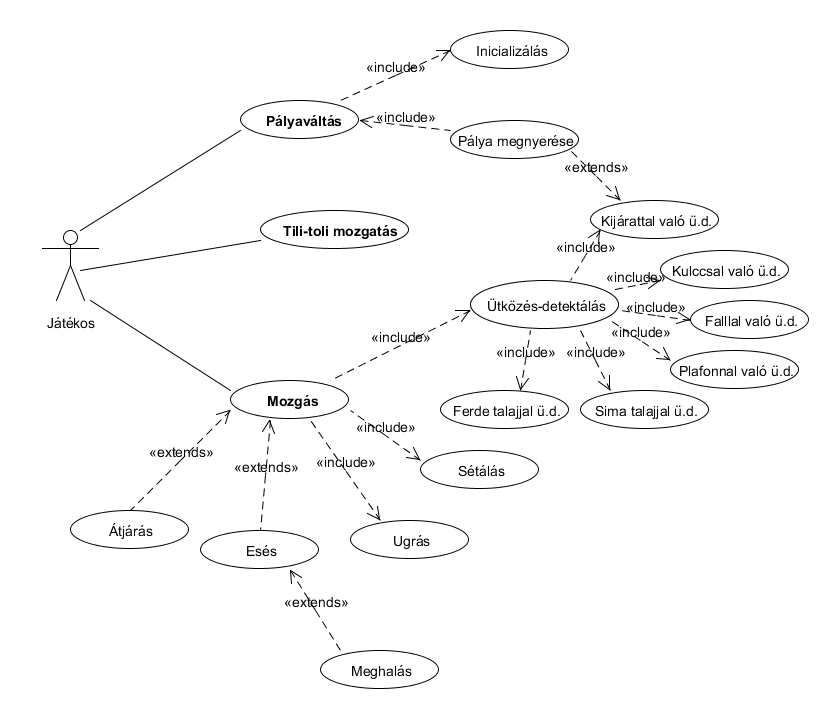
\includegraphics[scale=0.65,angle=90]{05_Use-case.png}
\newpage
\end{center}

\subsubsection{Use-case leírások}
Amely use-case leírásánál nem szerepel az \textbf{Aktorok} rész, annál a \textbf{Player} az aktor. Az alábbi leírásoknál külön nincs feltüntetve a \textbf{Forgatókönyv} rész, mivel folytonos időben történik a játék működése, azaz a virtuális világban igen apró lépésközökkel történik az állapotot változásának számítása, így túl aprólékos és részletes lenne mindegyik forgatókönyv kifejtése. Ezért ezeket a \textbf{Szekvencia diagramok a belső működésre} című részben mutatjuk meg folyamatukban.

\begin{usecase}
	\usecaseentry{Use-case neve}{Inicializálás}
	\usecaseentry{Rövid leírás}{A játék inicializálásának folyamata. Minden pálya betöltésekor meghívódik. A pályához tartozó változók kezdő értékét állítja be, mint például, hogy hány kulcs található a pályán, objektumok kezdő pozíciója.}
\end{usecase}

\begin{usecase}
	\usecaseentry{Use-case neve}{Pályaváltás}
	\usecaseentry{Rövid leírás}{Egy pálya betöltését végzi. Amennyiben következő pályát töltünk be, az újabb betöltése előtt eldobja a régit. A pálya objektumba inicializáláskor betöltött értékek alapján létrehozza a megfelelő objektumokat a pályán: játékos, kulcs(ok), ajtó. Ha az utolsó pályát teljesítettük éppen, akkor értelemszerűen nem fog újabb pályát betölteni, hanem a játék végét jelző információkat fogja csak megjeleníteni.}
\end{usecase}

\begin{usecase}
	\usecaseentry{Use-case neve}{Pálya megnyerése}
	\usecaseentry{Rövid leírás}{Ha úgy ütközünk a kijárattal, hogy már az összes kulcsot felvettük, akkor az adott pályát megnyerjük, ekkor {\itshape Pályaváltás} következik be. Amikor megnyertük az utolsó pályát is, megnyerjük a teljes játékot. Ehhez mindenkor számon tartjuk egy egyszerű belső változóként, hogy éppen hanyadik pályánál tartunk. Ha a teljesített pálya sorszáma elérte a maximumot, nincs több pálya, a játékot sikeresen teljesítettük. Ennek folyományaként, ha elindítjuk a játékot, a következő pálya újfent az első pálya lesz.}
\end{usecase}

\begin{usecase}
	\usecaseentry{Use-case neve}{Kijárattal való ütközés}
	\usecaseentry{Rövid leírás}{Amikor a pálya állapotfrissítő Update metódusa fut, lekérdezi, hogy a játékos ütközik-e a kijárattal. Ha igen, megvizsgálja, hogy az összes kulcs fel van-e már véve. Ezt követően ennek tudatában dönt a szükséges további cselekvésekről. Ha még nem szereztük meg mindet, akkor semmit nem csinál, egyszerűen ugyanúgy megy tovább a játék. Azonban, ha már felvettük mindet, és úgy érintkezünk a kijárattal, akkor életbe lép a {\itshape Pályaváltás} use-case.}
\end{usecase}

\begin{usecase}
	\usecaseentry{Use-case neve}{Tili-toli mozgatás}
	\usecaseentry{Rövid leírás}{A pályaelemeket lehetőségünk van mozgatni azért, hogy képesek legyünk átjárni pályaelemek között. Azok a szomszédos pályaelemek illeszkednek egymáshoz, amelyeknél a közös oldalon a blokkok elrendezése megegyezik. Ennek lekérdezésére való a pályaelemek IsPassableTo() metódusa, mely belül pont ezen tömböket hasonlítja össze. A pályaelemeket úgy tudnak mozogni, hogy a teljes pályát felosztjuk kisebb részekre, és egy helyet üresen hagyunk. A pályaelemek ezen üres helyre tudnak odébb mozogni. Ezen módszerrel lehetséges átrendezni sorrendjüket, hogy illeszkedő részeket tehessünk egymás mellé.}
\end{usecase}

\begin{usecase}
	\usecaseentry{Use-case neve}{Mozgás}
	\usecaseentry{Rövid leírás}{A pálcikaemberünket tudjuk közvetlenül irányítani, ő a játékosunk. Képes különböző mozgásokra, például sétálás, ugrás. A játékost mozgatva kell összeszedni a kulcsokat, majd a kijáratot elérni. Minden mozgás folyamán folytonos időben vizsgáljuk a haladást. Ez annyit tesz, hogy nagyon kis lépésközökre számítjuk a helyzetét. }
\end{usecase}

\begin{usecase}
	\usecaseentry{Use-case neve}{Átjárás}
	\usecaseentry{Rövid leírás}{Ha pontosan illeszkedő pályaelem kerül a pálcikaembert tartalmazó mellé, lehetőségünk van átjárni köztük. Ez az egyik legfontosabb mozgásfajta a játékban, mivel alapvetően logikai típusba sorolható a játéknem, és a tili-toli pont ezt szolgálja.}
\end{usecase}

\begin{usecase}
	\usecaseentry{Use-case neve}{Esés}
	\usecaseentry{Rövid leírás}{Amikor a pálcikaember mozgása során olyan részre érkezik, hogy nincs alatta talaj, elkezd zuhanni, esni. Ennek folyománya lehet a {\itshape Meghalás}. Az esés is egyfajta mozgás, viszont ezt nem a felhasználó kezdeményezi közvetlenül. Az esés folyamán is állandó jelleggel vizsgáljuk, hogy van-e alatta valami olyan felület, amibe tud ütközni. Ha van, értelemszerűen abba marad az esés és megáll az adott objektumon, talajon. Ha nincs akkor zuhan tovább. Abban az esetben, amikor egy lyukban zuhanva elértük a pályaelem szélét, két dolog lehetséges: van alattunk illeszkedő pályaelem, ekkor átlépünk arra; illetve ha nincs, akkor "kizuhanunk" a pályaelemből és a {\itshape Meghalás} use-case lép életbe.}
\end{usecase}

\newpage
\begin{usecase}
	\usecaseentry{Use-case neve}{Meghalás}
	\usecaseentry{Rövid leírás}{Amikor a játékos "kizuhan" a pályaelemből, akkor meghal. Ezt követően a játékos visszakerül az adott pályán az eredeti kiindulási pozíciójába, és a pályaelemek is visszarendeződnek eredeti helyükre. Annyiban különbözik a pálya teljes újrakezdésétől, hogy a már megszerzett kulcsokat nem kell újonnan felvenni. A játékos végtelen mennyiségben újraszülethet.}
\end{usecase}

\begin{usecase}
	\usecaseentry{Use-case neve}{Ugrás}
	\usecaseentry{Rövid leírás}{A talajon állva képes a játékos ugrani, amennyiben van elegendő helye ehhez. Ha annyi helye van, hogy legalább elkezdhesse, de ahhoz már kevés, hogy maximális magasságig felemelkedjen, akkor azon magasságig emelkedik, majd arról a tárgyról visszapattan. Míg a levegőben van a játékos, nem tudjuk irányítani, sem oldalirányba elmozdíttatni, sem pedig újabb ugrást kezdeményezni. Amíg valamilyen módon véget nem ér az ugrás folyamata, addig nem tudunk újabb pancsot adni neki.}
\end{usecase}

\begin{usecase}
	\usecaseentry{Use-case neve}{Sétálás}
	\usecaseentry{Rövid leírás}{Az egyik mozgásfajta, amit a felhasználó tud közvetlenül előidézni. A pálcikaember a talajon tud közlekedni, legyen az sima vagy ferde: a blokkokon mozog. Ahhoz, hogy ezt meg tudja tenni, folyamatos ütközésvizsgálat történik a kétfajta talajjal: simával és ferdével. Ezen ütközés-detektáló use-case alapján tud stabilan rajta maradni a talajon és nem pedig átesni rajta.}
\end{usecase}

\begin{usecase}
	\usecaseentry{Use-case neve}{Ütközés-detektálás}
	\usecaseentry{Rövid leírás}{A játékos befoglaló téglalapjának és a játéktéren elérhető objektumok kiterjedését reprezentáló befoglaló alakzatoknak a metszetének mértéke alapján történik az ütközés detektálás. Amennyiben a két terület metszete nem üres halmaz, igaz az eredmény, és a metszet területéből visszaszámítva kapunk egy vektort a metszés nagyságának függvényében. Ezt a vektort használjuk arra, hogy az objektum pozícióját korrigáljuk azért, hogy a felhasználó számára úgy tűnjön, hogy ténylegesen folytonos értékek alapján történik az ütközés detektálása. Így jobban közelítjük a valódi világ viselkedését, például a játékos nem tud belemenni a falba.}
\end{usecase}

\newpage
\begin{usecase}
	\usecaseentry{Use-case neve}{Ferde talajjal való ütközés-detektálás}
	\usecaseentry{Rövid leírás}{A ferde talaj (lejtő) annyiban különbözik a faltól, hogy ha oldalirányból ütközünk vele, akkor nem állunk meg, hanem felmehetünk rajta, míg ráesve a sima talajhoz hasonlóan viselkedik (megállunk a tetején).}
\end{usecase}

\begin{usecase}
	\usecaseentry{Use-case neve}{Sima talajjal való ütközés-detektálás}
	\usecaseentry{Rövid leírás}{{\itshape Esés} közben ha blokkal ütközünk, akkor azt a vízszintes teteje miatt sima talajként érzékeljük. Ekkor a {\itshape Fallal való ütközés}hez hasonlóan megállunk, nem esünk át rajta.}
\end{usecase}

\begin{usecase}
	\usecaseentry{Use-case neve}{Plafonnal való ütközés-detektálás}
	\usecaseentry{Rövid leírás}{Ugrást követően a vertikális elmozdulás mértékét az szabja meg, hogy van-e elég helyünk az ugrásra. Ha van, akkor a megadott magasságig felemelkedünk, majd visszaérkezünk a talajra. Ha viszont kevesebb a helyünk, azaz közel van a plafon, akkor azzal ütközve lepattanunk róla.}
\end{usecase}

\begin{usecase}
	\usecaseentry{Use-case neve}{Fallal való ütközés-detektálás}
	\usecaseentry{Rövid leírás}{Amikor oldalirányból ütközünk egy (nem ferde) blokkal -fallal-, akkor nem tudunk átmenni rajta, megállítja a pálcikaembert.}
\end{usecase}

\begin{usecase}
	\usecaseentry{Use-case neve}{Kulccsal való ütközés detektálás}
	\usecaseentry{Rövid leírás}{A pálya Update függvényének meghívásakor, ha a játékos olyan pozícióban áll, ahol érintkezik a kulccsal, akkor a pálya eltünteti a kulcsot a helyéről. A pályát csak akkor fejezhetjük be, ha minden kulcs helye üres.}
\end{usecase}
\pagebreak 
\subsection{Architektúra}

	A modellünk definiálásakor a valós-idejű élmény nyújtását fontosnak tekintettük, így rendkívül sok Player-, illetve Level Update fut le egymás után. Ez a felépítés a tesztesetek metódushívásonként történő naplózását teljesen áttekinthetetlenné tenné, ezért a tesztesetek statikusak.

	A tesztprogram futásakor a következő 4 teszteset közül választhatunk:
	\subsubsection{Első teszteset: Inicializálás}
	Pályaelemek, blokkok, avatár, kijárat, és kulcsok betöltése a 5.4.1 Játék inicializálás c. szekvenciadiagram alapján. 
	
	Tesztelt Use-Case-ek:
	
	-Inicializálás, 
	
	-Pályaváltás
	
	\subsubsection{Második teszteset: Pályaelem mozgatása}
	A 5.4.2 Illeszkedésvizsgálat illetve a 5.4.3 Csúsztatásvizsgálat c. szekvenciadiagram alapján tesztelt Use-case-ek: 
	
	-Tili-toli mozgatás
	
	\subsubsection{Harmadik teszteset: Játékos mozgás}
	Az avatár mozgásának, és az ütközések ellenőrzése a 5.4.4 Ütközésvizsgálat, illetve a 5.4.5 Játékos mozgása c. szekvenciadiagram alapján.
	
	Tesztelt Use-Case-ek: 
	
	-Átjárás, 
	
	-Mozgás, 
	
	-Esés, 
	
	-Meghalás, 
	
	-Ugrás, 
	
	-Sétálás, 
	
	-Ütközés-detektálás, 
	
	-Ferde talajjal való ütközés-detektálás, 
	
	-Sima talajjal való ütközés-detektálás, 
	
	-Plafonnal való ütközés-detektálás, 
	
	-Fallal való ütközés-detektálás
	
	\subsubsection{Negyedik teszteset: Pálya frissítés}
	A kulcsok, a győzelem, élet s halál ellenőrzése az 5.4.6 Pálya frissítése c. szekvenciadiagram alapján.
	
	Tesztelt Use-Case-ek: 
	
	-Pálya megnyerése, 
	
	-Kijárattal való ütközés, 
	
	-Kulccsal való ütközés detektálás, 
	
	-Pálya váltás
	
\subsection{A szkeleton kezelői felületének terve, dialógusok}

A szkeleton egy egyszerű konzolos alkalmazás lesz ami egy kérdéssel kezdődik arról, hogy melyik tesztesetet szeretnénk látni a négyből. A választás után a futás teljes eredménye kiíródik a képernyőre.

Mivel a modell úgy van megtervezve, hogy a virtuális világot nagyon kicsi időszeletekben szimulálja, a játék egy egyszerű mozzanatának végigkövetése is rengeteg ismétlődő függvény-hívásból állna. Ezt az eredmények átláthatósága miatt nem jelenítjük meg.

Emellett a különböző use-case-ek lefutása során csak minimális eltérés van a függvény-hívások szekvenciájában, így olyan általános futási eredményeket állítunk elő amik igazak több use-case-re is. Ezt a megfelelő helyre illesztett megjegyzésekkel fogjuk jelezni.

A modellünk jellegéből adódóan nincsenek dialógusok a szkeletonban, a felhasználó felé feltehető kérdések megfelelő kezelése nagyjából az algoritmusok implementálását jelentené. Mindezek fényében egy a következőhöz hasonló futást várunk a szkeletontól:

\begin{verbatim}
Level.slide(Direction direction)
|   // Find empty slot's XY coordinates.
|   // Get neighbour in the opposite of slide direction
|   // Swap the levelpart with the empty slot
|   // Call update on every levelpart
| - LevelPart.update()
|   | - this.neighbours[Direction.Left] = getNeighbour(Direction.Left)
|   |   |   // Calculate coordinates of levelpart by direction
|   |   | - return this.levelParts[x][y];
|   | - this.passabilities[Direction.Left] = isPassable(Direction.Left)
|   |   | - Boolean[] thisSide = this.getSide(direction)
|   |   | - Boolean[] otherSide = this.neighbours[direction]
|   |   |                                .getSide(oppositeDirection);
|   |   |   // check equality, return true/false
|   |   // Repeat this for the other directions
\end{verbatim}

\subsection{Szekvencia diagramok a belső működésre}
	\subsubsection{Játék inicializálása}
		\begin{center}
		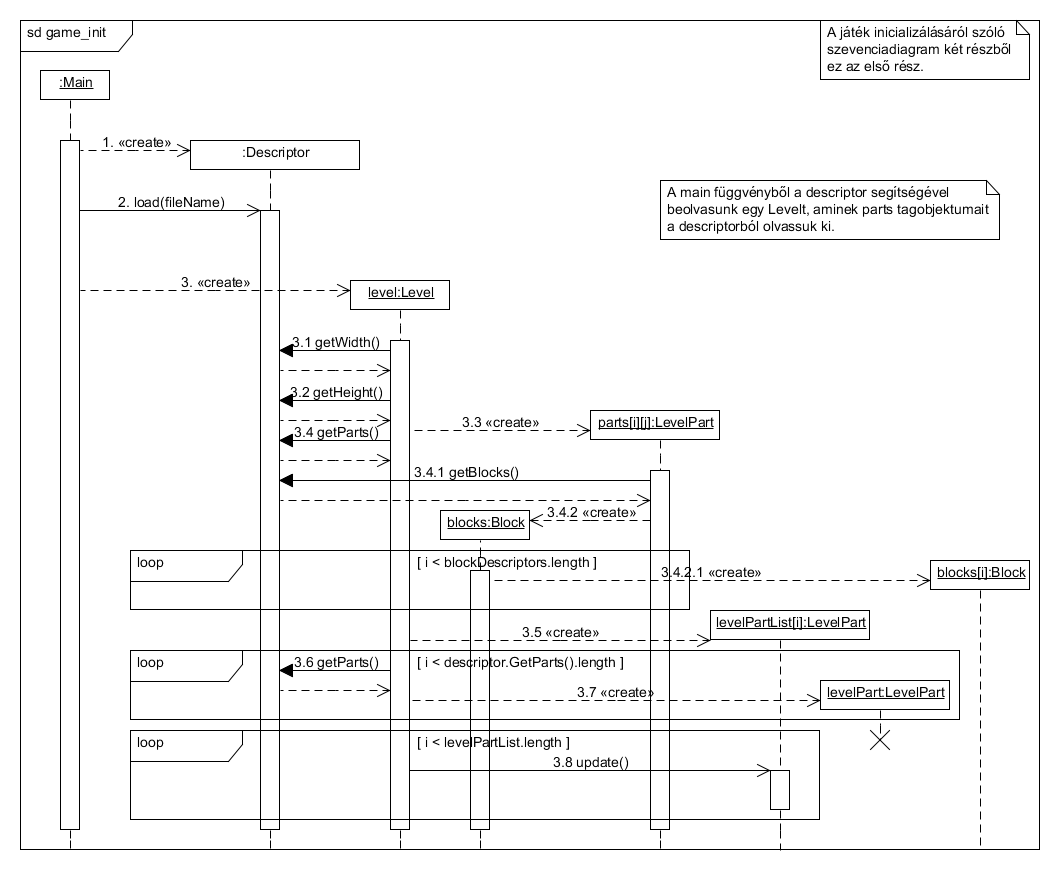
\includegraphics[scale=0.51,angle=90]{05_sdGameInita.png}
		\newpage
		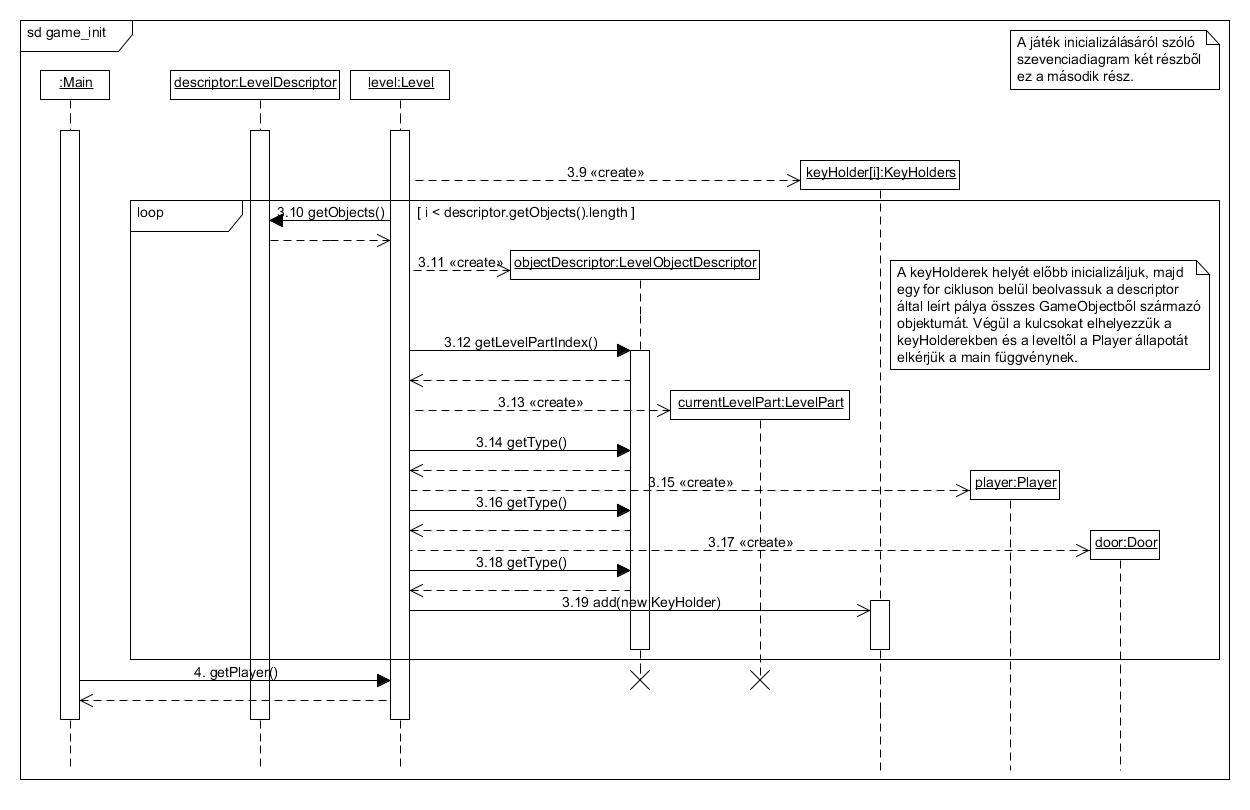
\includegraphics[scale=0.50,angle=90]{03_sdGameInitb.png}
		\newpage
		\end{center}
	\subsubsection{Illeszkedésvizsgálat}
		\begin{center}
		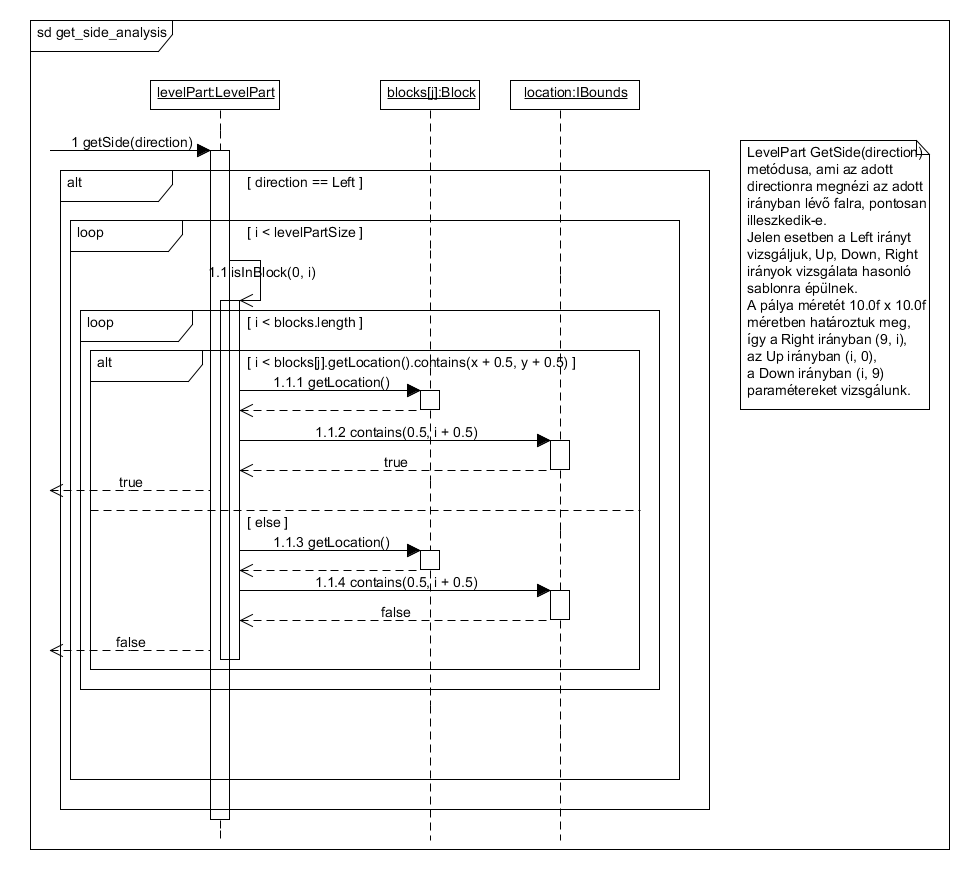
\includegraphics[scale=0.46]{03_sdGetSideAnalysis.png}
		\newpage
		\end{center}
	\subsubsection{Csúsztatásvizsgálat}
		\begin{center}
		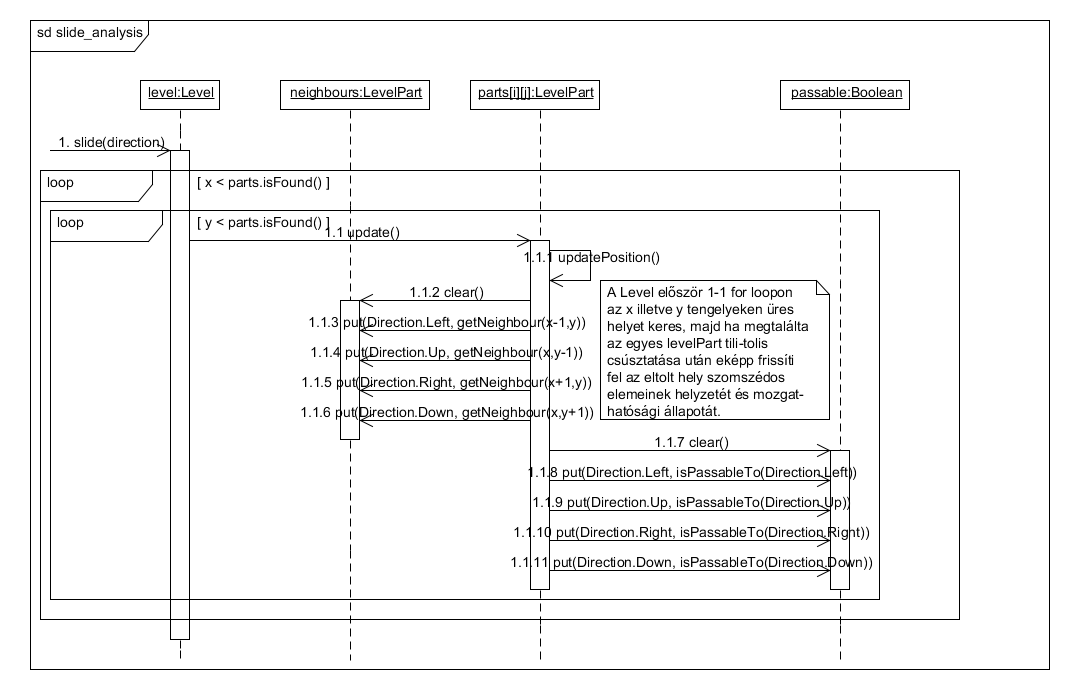
\includegraphics[scale=0.60,angle=90]{03_sdSlideAnalysis.png}
		\newpage
		\end{center}
	\subsubsection{Ütközésvizsgálat}
		\begin{center}
		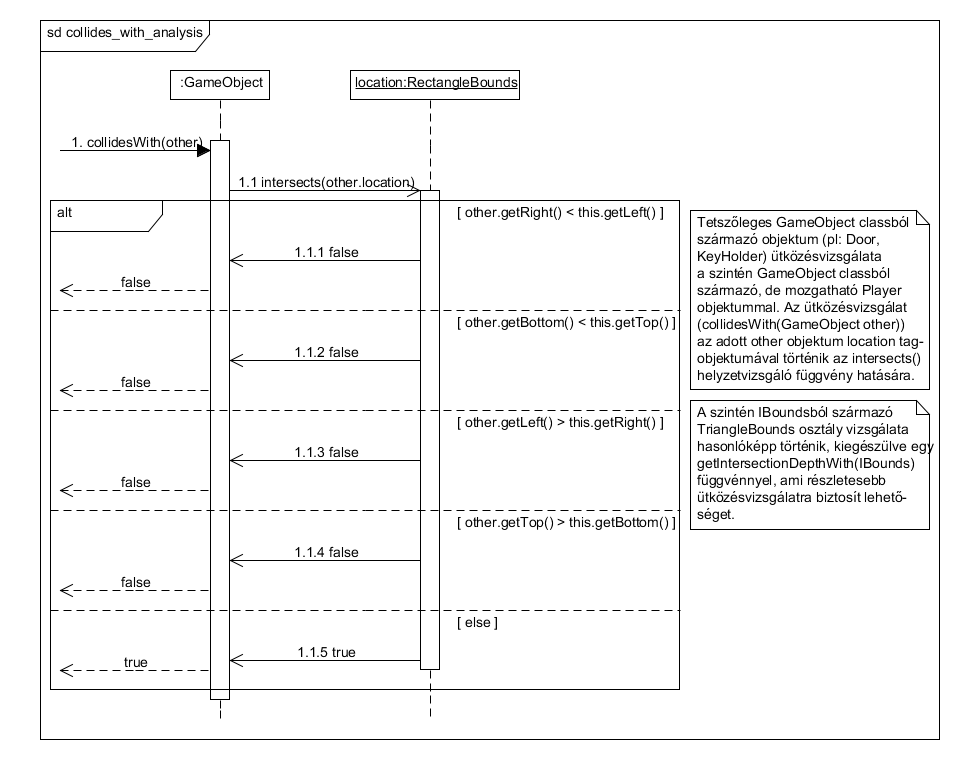
\includegraphics[scale=0.47]{03_sdCollidesWithAnalysis.png}
		\end{center}
	\subsubsection{Játékos mozgatása}
		\begin{center}
		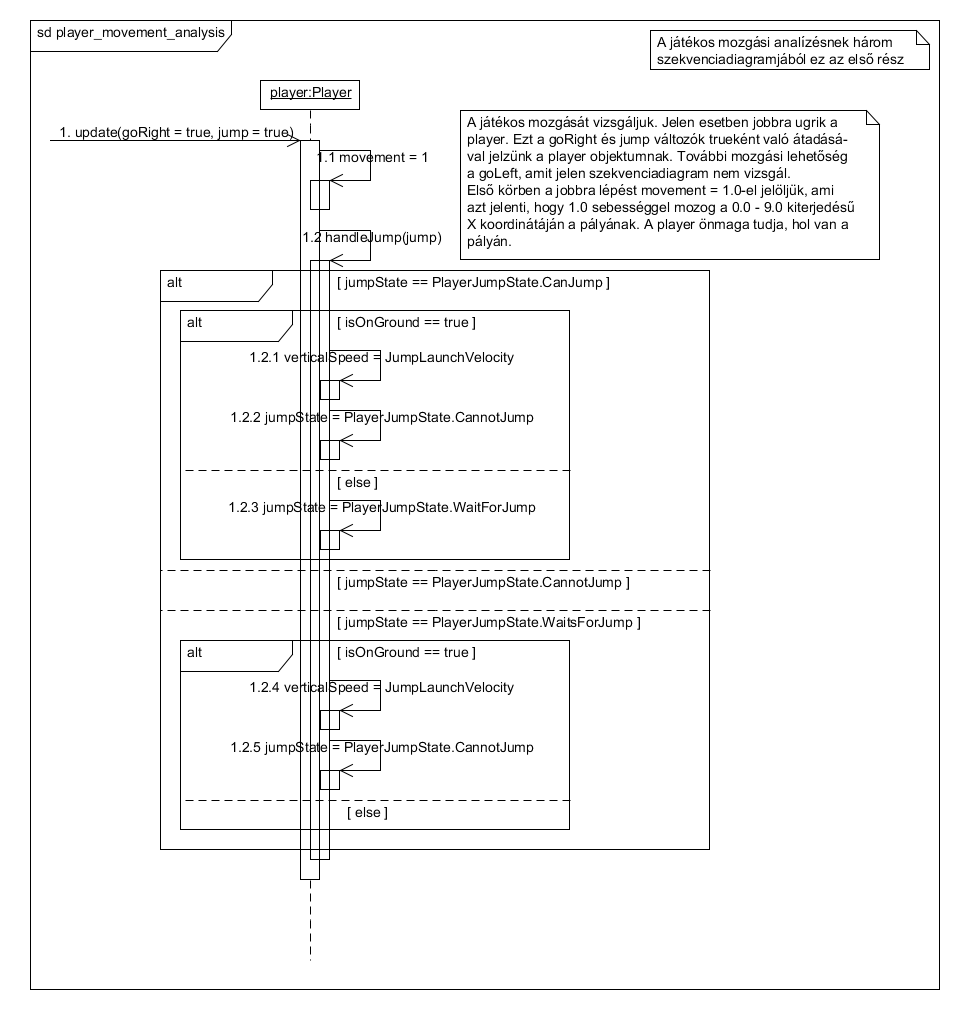
\includegraphics[scale=0.40]{03_sdPlayerMovementAnalysisa.png}
		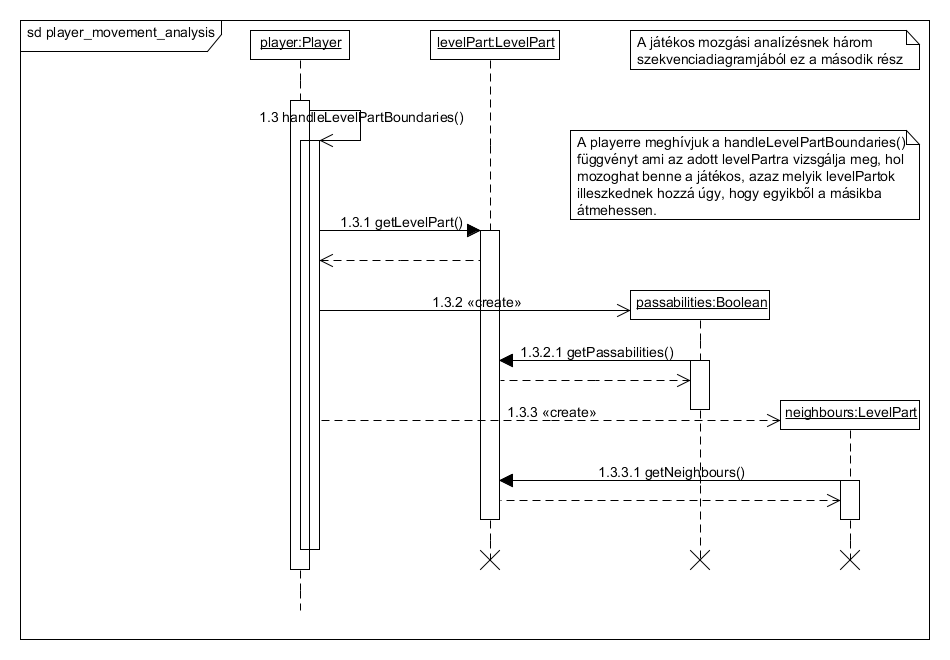
\includegraphics[scale=0.40]{03_sdPlayerMovementAnalysisb.png}
		\newpage
		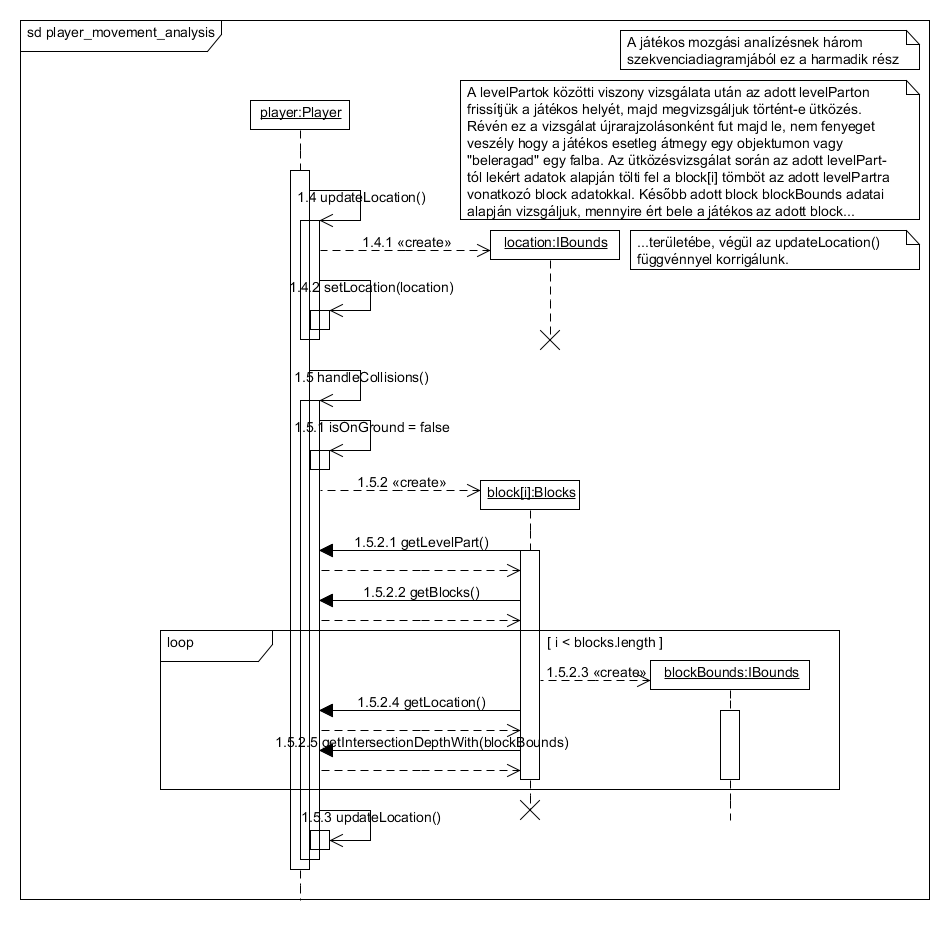
\includegraphics[scale=0.45]{03_sdPlayerMovementAnalysisc.png}
		\newpage
		\end{center}
	\subsubsection{Pálya frissítése}
		\begin{center}
		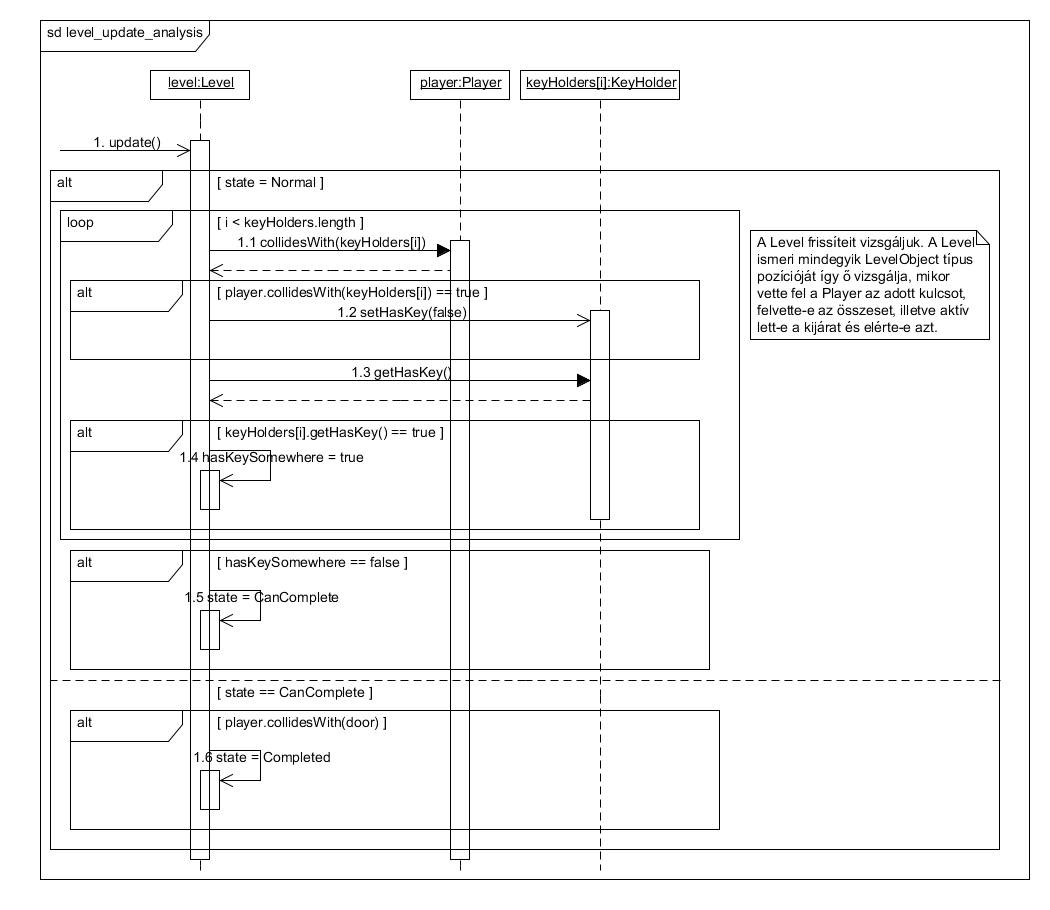
\includegraphics[scale=0.42]{05_sdLevelUpdateAnalysis.png}
		\newpage
		\end{center}

\subsection{Napló}

\begin{journal}

\journalentry{2012.03.07. 12:30}{1}{Biró, Kanyó, Magyar, Tarjáni, Vajsz}{Személyes értekezlet. A konzultáció tapasztalatait megbeszéltük, felosztottuk a feladatokat, kijelöltük az általános irányvonalat a munkához.}

\journalentry{2012.03.07. 16:00}{1,5}{Biró}{Terveztem és ötleteket gyűjtöttem a szkeleton tervéhez.}
\journalentry{2012.03.10. 13:00}{2}{Tarjáni}{Use-case diagram elkészítése, a dokumentumba szerkesztése.}
\journalentry{2012.03.10. 19:00}{4}{Kanyó}{Sablon készítése a Use-case leírásokhoz, majd a leírások készítése.}
\journalentry{2012.03.10. 20:00}{1,5}{Biró}{Teszteseteket terveztem és kitaláltam a kiírás formátumát.}
\journalentry{2012.03.10. 20:20}{4,5}{Magyar}{Tesztesetek tervezése, egyeztetése szekvenciadiagramokkal, architektúra szekció összefoglalása, formázás javítás.}
\journalentry{2012.03.11. 9:30}{2,5}{Kanyó}{Use-case leírások készítése.}
\journalentry{2012.03.11. 19:30}{3}{Tarjáni}{Use-case diagram átalakítása, a use-case leírások ellenőrzése, helyenként szerkesztése, a hiányzó leírások megírása.}
\journalentry{2012.03.11. 20:00}{1}{Biró}{Megírtam a szkeleton kezelői felületének terve fejezetet.}
\journalentry{2012.03.11. 21:15}{1,5}{Vajsz}{Szekvenciadiagramok felülvizsgálata és frissítése}

\end{journal}

\end{document}